\documentclass[]{article}
\usepackage{lmodern}
\usepackage{amssymb,amsmath}
\usepackage{ifxetex,ifluatex}
\usepackage{fixltx2e} % provides \textsubscript
\ifnum 0\ifxetex 1\fi\ifluatex 1\fi=0 % if pdftex
  \usepackage[T1]{fontenc}
  \usepackage[utf8]{inputenc}
\else % if luatex or xelatex
  \ifxetex
    \usepackage{mathspec}
  \else
    \usepackage{fontspec}
  \fi
  \defaultfontfeatures{Ligatures=TeX,Scale=MatchLowercase}
\fi
% use upquote if available, for straight quotes in verbatim environments
\IfFileExists{upquote.sty}{\usepackage{upquote}}{}
% use microtype if available
\IfFileExists{microtype.sty}{%
\usepackage{microtype}
\UseMicrotypeSet[protrusion]{basicmath} % disable protrusion for tt fonts
}{}
\usepackage[margin=1in]{geometry}
\usepackage{hyperref}
\hypersetup{unicode=true,
            pdftitle={Trabalho de dados Binários},
            pdfauthor={Laís Hoffmann, Simone Matsubara, Yasmin Fernandes, Willian Meira},
            pdfborder={0 0 0},
            breaklinks=true}
\urlstyle{same}  % don't use monospace font for urls
\usepackage{color}
\usepackage{fancyvrb}
\newcommand{\VerbBar}{|}
\newcommand{\VERB}{\Verb[commandchars=\\\{\}]}
\DefineVerbatimEnvironment{Highlighting}{Verbatim}{commandchars=\\\{\}}
% Add ',fontsize=\small' for more characters per line
\usepackage{framed}
\definecolor{shadecolor}{RGB}{248,248,248}
\newenvironment{Shaded}{\begin{snugshade}}{\end{snugshade}}
\newcommand{\KeywordTok}[1]{\textcolor[rgb]{0.13,0.29,0.53}{\textbf{{#1}}}}
\newcommand{\DataTypeTok}[1]{\textcolor[rgb]{0.13,0.29,0.53}{{#1}}}
\newcommand{\DecValTok}[1]{\textcolor[rgb]{0.00,0.00,0.81}{{#1}}}
\newcommand{\BaseNTok}[1]{\textcolor[rgb]{0.00,0.00,0.81}{{#1}}}
\newcommand{\FloatTok}[1]{\textcolor[rgb]{0.00,0.00,0.81}{{#1}}}
\newcommand{\ConstantTok}[1]{\textcolor[rgb]{0.00,0.00,0.00}{{#1}}}
\newcommand{\CharTok}[1]{\textcolor[rgb]{0.31,0.60,0.02}{{#1}}}
\newcommand{\SpecialCharTok}[1]{\textcolor[rgb]{0.00,0.00,0.00}{{#1}}}
\newcommand{\StringTok}[1]{\textcolor[rgb]{0.31,0.60,0.02}{{#1}}}
\newcommand{\VerbatimStringTok}[1]{\textcolor[rgb]{0.31,0.60,0.02}{{#1}}}
\newcommand{\SpecialStringTok}[1]{\textcolor[rgb]{0.31,0.60,0.02}{{#1}}}
\newcommand{\ImportTok}[1]{{#1}}
\newcommand{\CommentTok}[1]{\textcolor[rgb]{0.56,0.35,0.01}{\textit{{#1}}}}
\newcommand{\DocumentationTok}[1]{\textcolor[rgb]{0.56,0.35,0.01}{\textbf{\textit{{#1}}}}}
\newcommand{\AnnotationTok}[1]{\textcolor[rgb]{0.56,0.35,0.01}{\textbf{\textit{{#1}}}}}
\newcommand{\CommentVarTok}[1]{\textcolor[rgb]{0.56,0.35,0.01}{\textbf{\textit{{#1}}}}}
\newcommand{\OtherTok}[1]{\textcolor[rgb]{0.56,0.35,0.01}{{#1}}}
\newcommand{\FunctionTok}[1]{\textcolor[rgb]{0.00,0.00,0.00}{{#1}}}
\newcommand{\VariableTok}[1]{\textcolor[rgb]{0.00,0.00,0.00}{{#1}}}
\newcommand{\ControlFlowTok}[1]{\textcolor[rgb]{0.13,0.29,0.53}{\textbf{{#1}}}}
\newcommand{\OperatorTok}[1]{\textcolor[rgb]{0.81,0.36,0.00}{\textbf{{#1}}}}
\newcommand{\BuiltInTok}[1]{{#1}}
\newcommand{\ExtensionTok}[1]{{#1}}
\newcommand{\PreprocessorTok}[1]{\textcolor[rgb]{0.56,0.35,0.01}{\textit{{#1}}}}
\newcommand{\AttributeTok}[1]{\textcolor[rgb]{0.77,0.63,0.00}{{#1}}}
\newcommand{\RegionMarkerTok}[1]{{#1}}
\newcommand{\InformationTok}[1]{\textcolor[rgb]{0.56,0.35,0.01}{\textbf{\textit{{#1}}}}}
\newcommand{\WarningTok}[1]{\textcolor[rgb]{0.56,0.35,0.01}{\textbf{\textit{{#1}}}}}
\newcommand{\AlertTok}[1]{\textcolor[rgb]{0.94,0.16,0.16}{{#1}}}
\newcommand{\ErrorTok}[1]{\textcolor[rgb]{0.64,0.00,0.00}{\textbf{{#1}}}}
\newcommand{\NormalTok}[1]{{#1}}
\usepackage{graphicx,grffile}
\makeatletter
\def\maxwidth{\ifdim\Gin@nat@width>\linewidth\linewidth\else\Gin@nat@width\fi}
\def\maxheight{\ifdim\Gin@nat@height>\textheight\textheight\else\Gin@nat@height\fi}
\makeatother
% Scale images if necessary, so that they will not overflow the page
% margins by default, and it is still possible to overwrite the defaults
% using explicit options in \includegraphics[width, height, ...]{}
\setkeys{Gin}{width=\maxwidth,height=\maxheight,keepaspectratio}
\IfFileExists{parskip.sty}{%
\usepackage{parskip}
}{% else
\setlength{\parindent}{0pt}
\setlength{\parskip}{6pt plus 2pt minus 1pt}
}
\setlength{\emergencystretch}{3em}  % prevent overfull lines
\providecommand{\tightlist}{%
  \setlength{\itemsep}{0pt}\setlength{\parskip}{0pt}}
\setcounter{secnumdepth}{0}
% Redefines (sub)paragraphs to behave more like sections
\ifx\paragraph\undefined\else
\let\oldparagraph\paragraph
\renewcommand{\paragraph}[1]{\oldparagraph{#1}\mbox{}}
\fi
\ifx\subparagraph\undefined\else
\let\oldsubparagraph\subparagraph
\renewcommand{\subparagraph}[1]{\oldsubparagraph{#1}\mbox{}}
\fi

%%% Use protect on footnotes to avoid problems with footnotes in titles
\let\rmarkdownfootnote\footnote%
\def\footnote{\protect\rmarkdownfootnote}

%%% Change title format to be more compact
\usepackage{titling}

% Create subtitle command for use in maketitle
\newcommand{\subtitle}[1]{
  \posttitle{
    \begin{center}\large#1\end{center}
    }
}

\setlength{\droptitle}{-2em}

  \title{Trabalho de dados Binários}
    \pretitle{\vspace{\droptitle}\centering\huge}
  \posttitle{\par}
  \subtitle{Acidentes de carro}
  \author{Laís Hoffmann, Simone Matsubara, Yasmin Fernandes, Willian Meira}
    \preauthor{\centering\large\emph}
  \postauthor{\par}
      \predate{\centering\large\emph}
  \postdate{\par}
    \date{2018-11-11}

\usepackage[brazil]{babel} \usepackage{amsmath} \usepackage{float}
\usepackage{bm}

\begin{document}
\maketitle

\section{1. Base de Dados}\label{base-de-dados}

\textbf{1.1 Descrição dos dados}

Os dados foram retirados do pacote ``DAAG'', sendo dados dos EUA, entre
1997-2002, de acidentes de carro relatados pela polícia nos quais há um
evento prejudicial (pessoas ou propriedade) e do qual pelo menos um
veículo foi rebocado. Os dados são restritos aos ocupantes do banco da
frente, incluem apenas um subconjunto das variáveis registradas e são
restritos de outras maneiras também.

A base original possui uma base de dados com 26.217 observações nas 15
variáveis a seguir.

1 - \textbf{veloc}: velocidades estimadas do impacto do acidente:
1-9km/h, 10-24, 25-39, 40-54, 55+ \newline 2 - \textbf{pesos}: Pesos de
observação \newline 3 - \textbf{sobrev}: Classificação se sobreviveu ao
acidente: 1 = morreu ou 0 = sobreviveu \newline 4 - \textbf{airbag}: Se
o carro possui airbag: com ou sem airbag \newline 5 - \textbf{cinto}:
uso do cinto de segurança: com ou sem cinto \newline 6 -
\textbf{frontal}: impacto do acidente: 0 = não frontal, 1 = impacto
frontal \newline 7 - \textbf{sexo}: Sexo: 0 = Feminino ou 1 = Masculino
\newline 8 - \textbf{idade}: Idade dos ocupantes do veículo \newline 9 -
\textbf{anoaci}: Ano do acidente (1997-2002) \newline 10 -
\textbf{anovei}: Ano do veículo (1953-2003) \newline 11 -
\textbf{airbagcat}: Se Airbags foram acionados: deploy, nodeploy,
unavail \newline 12 - \textbf{ocupantes}: Posição do airbag acionado:
driver, pass \newline 13 - \textbf{abfunc}: Airbag acionados: 0: Se não
possuia airbag ou não foi acionado, 1: Um ou mais airbags foram
acionados \newline 14 - \textbf{grav}: Gravidade do acidente: 0:none, 1
= Possível Lesão, 2:no incapacity, 3:incapacity, 4:killed; 5:unknown,
6:prior death \newline 15 - \textbf{numcaso}: Número do caso.

No entanto, escolhemos analisar os dados do ano do acidente de 2002 e
veículos de ano 2000 e retirar as variaveis weight, abcat e caseid.

\section{2 Análise Descritiva}\label{analise-descritiva}

\textbf{2.1 Medidas de Resumo}

\begin{Shaded}
\begin{Highlighting}[]
\KeywordTok{summary}\NormalTok{(dados[ , }\KeywordTok{c}\NormalTok{(}\DecValTok{1}\NormalTok{:}\DecValTok{8}\NormalTok{,}\DecValTok{10}\NormalTok{)])}
\end{Highlighting}
\end{Shaded}

\begin{verbatim}
##        veloc         sobrev           airbag          cinto       
##  01-09 mph: 12   Min.   :0.0000   Min.   :0.000   Min.   :0.0000  
##  10-24 mph:293   1st Qu.:1.0000   1st Qu.:1.000   1st Qu.:1.0000  
##  25-39 mph:121   Median :1.0000   Median :1.000   Median :1.0000  
##  40-54 mph: 46   Mean   :0.9533   Mean   :0.998   Mean   :0.7546  
##  55+ mph  : 21   3rd Qu.:1.0000   3rd Qu.:1.000   3rd Qu.:1.0000  
##                  Max.   :1.0000   Max.   :1.000   Max.   :1.0000  
##                                                                   
##     frontal         sexo         idade         ocupantes       grav    
##  Min.   :0.0000   Fem :254   Min.   :16.00   Min.   :0.000   0   :145  
##  1st Qu.:0.0000   Masc:239   1st Qu.:23.00   1st Qu.:1.000   1   :102  
##  Median :1.0000              Median :35.00   Median :1.000   2   : 81  
##  Mean   :0.6288              Mean   :37.82   Mean   :0.783   3   :139  
##  3rd Qu.:1.0000              3rd Qu.:48.00   3rd Qu.:1.000   4   : 19  
##  Max.   :1.0000              Max.   :93.00   Max.   :1.000   5   :  3  
##                                                              NA's:  4
\end{verbatim}

\textbf{2.3 Histogramas}

\begin{Shaded}
\begin{Highlighting}[]
\KeywordTok{par}\NormalTok{(}\DataTypeTok{mfrow =} \KeywordTok{c}\NormalTok{(}\DecValTok{3}\NormalTok{,}\DecValTok{3}\NormalTok{))}
\KeywordTok{plot}\NormalTok{(dados$abfunc, }\DataTypeTok{xlab =} \StringTok{''}\NormalTok{, }\DataTypeTok{ylab =} \StringTok{''}\NormalTok{, }\DataTypeTok{main =} \StringTok{'AB Funcionou'}\NormalTok{)}
\KeywordTok{plot}\NormalTok{(dados$veloc, }\DataTypeTok{xlab =} \StringTok{''}\NormalTok{, }\DataTypeTok{ylab =} \StringTok{''}\NormalTok{, }\DataTypeTok{main =} \StringTok{'Velocidade'}\NormalTok{)}
\KeywordTok{plot}\NormalTok{(dados$sobrev, }\DataTypeTok{xlab =} \StringTok{''}\NormalTok{, }\DataTypeTok{ylab =} \StringTok{''}\NormalTok{, }\DataTypeTok{main =} \StringTok{'Sobrevivente'}\NormalTok{)}
\KeywordTok{plot}\NormalTok{(dados$airbag, }\DataTypeTok{xlab =} \StringTok{''}\NormalTok{, }\DataTypeTok{ylab =} \StringTok{''}\NormalTok{, }\DataTypeTok{main =} \StringTok{'Airbag'}\NormalTok{)}
\KeywordTok{plot}\NormalTok{(dados$cinto, }\DataTypeTok{xlab =} \StringTok{''}\NormalTok{, }\DataTypeTok{ylab =} \StringTok{''}\NormalTok{, }\DataTypeTok{main =} \StringTok{'Cinto'}\NormalTok{)}
\KeywordTok{plot}\NormalTok{(dados$frontal, }\DataTypeTok{xlab =} \StringTok{''}\NormalTok{, }\DataTypeTok{ylab =} \StringTok{''}\NormalTok{, }\DataTypeTok{main =} \StringTok{'Frontal'}\NormalTok{)}
\KeywordTok{plot}\NormalTok{(dados$sexo, }\DataTypeTok{xlab =} \StringTok{''}\NormalTok{, }\DataTypeTok{ylab =} \StringTok{''}\NormalTok{, }\DataTypeTok{main =} \StringTok{'Sexo'}\NormalTok{)}
\KeywordTok{plot}\NormalTok{(dados$ocupantes, }\DataTypeTok{xlab =} \StringTok{''}\NormalTok{, }\DataTypeTok{ylab =} \StringTok{''}\NormalTok{, }\DataTypeTok{main =} \StringTok{'Ocupante'}\NormalTok{)}
\KeywordTok{plot}\NormalTok{(dados$grav, }\DataTypeTok{xlab =} \StringTok{''}\NormalTok{, }\DataTypeTok{ylab =} \StringTok{''}\NormalTok{, }\DataTypeTok{main =} \StringTok{'Gravidade'}\NormalTok{)}
\KeywordTok{mtext}\NormalTok{(}\DataTypeTok{side=}\DecValTok{2}\NormalTok{,}\DataTypeTok{cex=}\FloatTok{1.3}\NormalTok{,}\DataTypeTok{line=}\NormalTok{-}\FloatTok{1.5}\NormalTok{,}\DataTypeTok{text=}\StringTok{"Proporção das variaveis"}\NormalTok{,}\DataTypeTok{outer=}\OtherTok{TRUE}\NormalTok{)}
\end{Highlighting}
\end{Shaded}

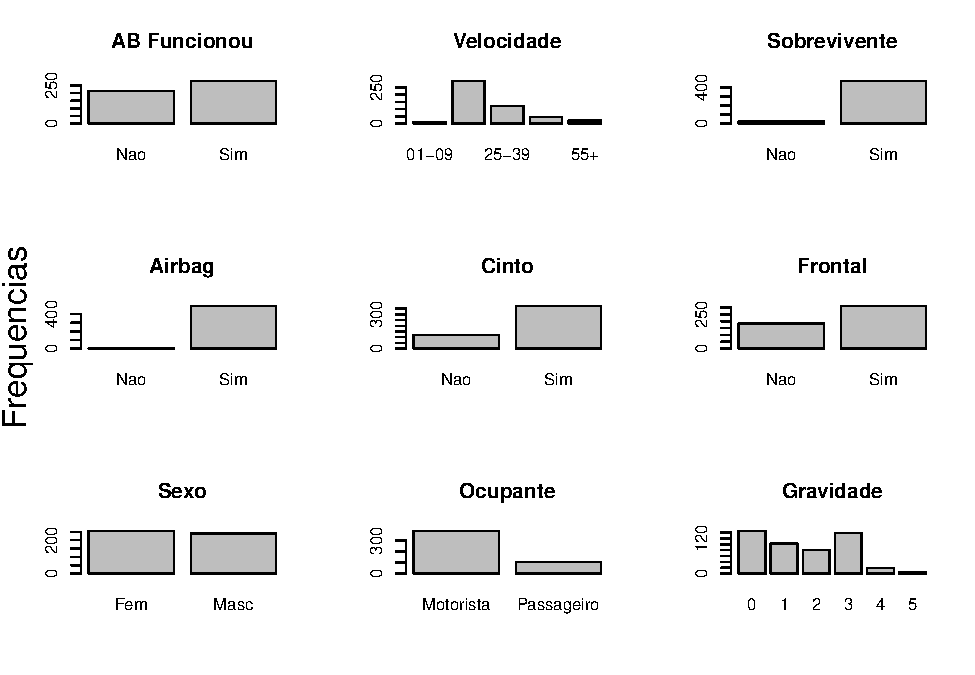
\includegraphics{Dados_Binários1_files/figure-latex/unnamed-chunk-5-1.pdf}

\textbf{2.4 Distribuição}

\begin{Shaded}
\begin{Highlighting}[]
\KeywordTok{grid.arrange}\NormalTok{(g1, g2, g3, g4, g5, g6, g7,g8, }\DataTypeTok{ncol=}\DecValTok{3}\NormalTok{, }\DataTypeTok{nrow=}\DecValTok{3}\NormalTok{)}
\end{Highlighting}
\end{Shaded}

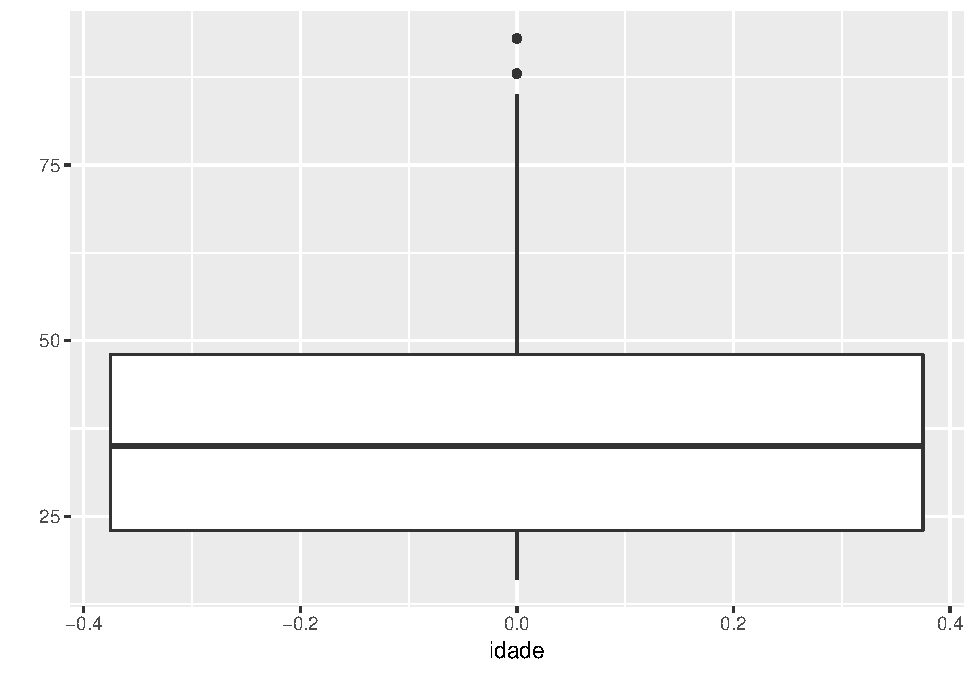
\includegraphics{Dados_Binários1_files/figure-latex/unnamed-chunk-7-1.pdf}

\textbf{2.5 Análise de correlações entre covariáveis}

\textbf{2.6 Gráficos de Disperção}

\begin{Shaded}
\begin{Highlighting}[]
\NormalTok{dis}
\end{Highlighting}
\end{Shaded}

\begin{verbatim}
## NULL
\end{verbatim}

\section{3. AJUSTE DO MODELO DE
REGRESSÃO}\label{ajuste-do-modelo-de-regressao}

\textbf{3.1 Ligação Logito}

\begin{Shaded}
\begin{Highlighting}[]
\NormalTok{ajuste1 <-}\StringTok{ }\KeywordTok{glm}\NormalTok{(abfunc ~}\StringTok{ }\NormalTok{.,}\DataTypeTok{family=}\KeywordTok{binomial}\NormalTok{(}\DataTypeTok{link=}\StringTok{'logit'}\NormalTok{),}\DataTypeTok{data =} \NormalTok{dados)}
\end{Highlighting}
\end{Shaded}

\textbf{3.2 Ligação Probito}

\begin{Shaded}
\begin{Highlighting}[]
\NormalTok{ajuste2 <-}\StringTok{ }\KeywordTok{glm}\NormalTok{(abfunc ~}\StringTok{ }\NormalTok{.,}\DataTypeTok{family=}\KeywordTok{binomial}\NormalTok{(}\DataTypeTok{link =} \StringTok{'probit'}\NormalTok{),}\DataTypeTok{data =} \NormalTok{dados)}
\end{Highlighting}
\end{Shaded}

\textbf{3.3 Ligação Complemento log-log}

\begin{Shaded}
\begin{Highlighting}[]
\NormalTok{ajuste3 <-}\StringTok{ }\KeywordTok{glm}\NormalTok{(abfunc ~}\StringTok{ }\NormalTok{.,}\DataTypeTok{family=}\KeywordTok{binomial}\NormalTok{(}\DataTypeTok{link=}\StringTok{'cloglog'}\NormalTok{),}\DataTypeTok{data =} \NormalTok{dados)}
\end{Highlighting}
\end{Shaded}

\textbf{3.4 Ligação Cauchy}

\begin{Shaded}
\begin{Highlighting}[]
\NormalTok{ajuste4 <-}\StringTok{ }\KeywordTok{glm}\NormalTok{(abfunc ~}\StringTok{ }\NormalTok{.,}\DataTypeTok{family=}\KeywordTok{binomial}\NormalTok{(}\DataTypeTok{link=}\StringTok{'cauchit'}\NormalTok{),}\DataTypeTok{data =} \NormalTok{dados)}
\end{Highlighting}
\end{Shaded}

\section{4. ESCOLHA DO MODELO}\label{escolha-do-modelo}

\begin{Shaded}
\begin{Highlighting}[]
\NormalTok{selec <-}\StringTok{ }\KeywordTok{data.frame}\NormalTok{(}\DataTypeTok{ajuste=}\KeywordTok{c}\NormalTok{(}\StringTok{'logito'}\NormalTok{, }\StringTok{'probito'}\NormalTok{, }\StringTok{'cloglog'}\NormalTok{, }\StringTok{'cauchy'}\NormalTok{),}
                    \DataTypeTok{aic=}\KeywordTok{c}\NormalTok{(}\KeywordTok{AIC}\NormalTok{(ajuste1), }\KeywordTok{AIC}\NormalTok{(ajuste2), }\KeywordTok{AIC}\NormalTok{(ajuste3), }\KeywordTok{AIC}\NormalTok{(ajuste4)),}
                    \DataTypeTok{logLik=}\KeywordTok{c}\NormalTok{(}\KeywordTok{logLik}\NormalTok{(ajuste1),}\KeywordTok{logLik}\NormalTok{(ajuste2),}\KeywordTok{logLik}\NormalTok{(ajuste3),}\KeywordTok{logLik}\NormalTok{(ajuste4)))}

\NormalTok{selec}
\end{Highlighting}
\end{Shaded}

\begin{verbatim}
##    ajuste      aic    logLik
## 1  logito 514.1660 -240.0830
## 2 probito 514.1476 -240.0738
## 3 cloglog 513.2723 -239.6361
## 4  cauchy 514.4334 -240.2167
\end{verbatim}

O modelo que apresentou menor AIC e maior verossimilhança foi o modelo
Binomial com função de ligação C Log-Log.

\section{5. ANÁLISE DO MODELO AJUSTADO
SELECIONADO}\label{analise-do-modelo-ajustado-selecionado}

\textbf{5.1 Resumo do Modelo}

\begin{Shaded}
\begin{Highlighting}[]
\KeywordTok{summary}\NormalTok{(ajuste4)}
\end{Highlighting}
\end{Shaded}

\begin{verbatim}
## 
## Call:
## glm(formula = abfunc ~ ., family = binomial(link = "cauchit"), 
##     data = dados)
## 
## Deviance Residuals: 
##     Min       1Q   Median       3Q      Max  
## -2.2170  -0.7038   0.4328   0.7398   2.5201  
## 
## Coefficients:
##               Estimate Std. Error z value Pr(>|z|)    
## (Intercept) -1.794e+05  4.762e+07  -0.004   0.9970    
## veloc.L      4.958e+00  3.475e+00   1.427   0.1536    
## veloc.Q     -3.154e+00  2.923e+00  -1.079   0.2805    
## veloc.C      5.688e-01  1.765e+00   0.322   0.7473    
## veloc^4     -8.876e-01  7.550e-01  -1.176   0.2398    
## sobrev      -2.501e+00  2.218e+00  -1.127   0.2596    
## airbag       1.794e+05  4.762e+07   0.004   0.9970    
## cinto       -7.841e-01  3.298e-01  -2.377   0.0174 *  
## frontal      3.124e+00  5.108e-01   6.116 9.61e-10 ***
## sexoMasc    -1.285e-01  2.512e-01  -0.511   0.6090    
## idade        2.668e-03  7.695e-03   0.347   0.7288    
## ocupantes    2.477e-01  3.258e-01   0.760   0.4472    
## grav.L      -1.672e+00  1.122e+00  -1.490   0.1362    
## grav.Q      -2.051e+00  8.045e-01  -2.549   0.0108 *  
## grav.C       1.334e+00  1.291e+00   1.033   0.3014    
## grav^4       2.100e+00  1.368e+00   1.535   0.1249    
## grav^5       9.909e-01  8.447e-01   1.173   0.2407    
## ---
## Signif. codes:  0 '***' 0.001 '**' 0.01 '*' 0.05 '.' 0.1 ' ' 1
## 
## (Dispersion parameter for binomial family taken to be 1)
## 
##     Null deviance: 670.27  on 488  degrees of freedom
## Residual deviance: 480.43  on 472  degrees of freedom
##   (4 observations deleted due to missingness)
## AIC: 514.43
## 
## Number of Fisher Scoring iterations: 17
\end{verbatim}

\textbf{5.2 Reajuste do Modelo}

\begin{Shaded}
\begin{Highlighting}[]
\NormalTok{ajuste4}\FloatTok{.1} \NormalTok{<-}\StringTok{ }\KeywordTok{step}\NormalTok{(ajuste4, }\DataTypeTok{direction =} \StringTok{"both"}\NormalTok{)}
\end{Highlighting}
\end{Shaded}

\begin{verbatim}
## Start:  AIC=514.43
## abfunc ~ veloc + sobrev + airbag + cinto + frontal + sexo + idade + 
##     ocupantes + grav
## 
##             Df Deviance    AIC
## - idade      1   480.53 512.53
## - sexo       1   480.69 512.69
## - ocupantes  1   481.09 513.09
## <none>           480.43 514.43
## - airbag     1   482.53 514.53
## - sobrev     1   482.77 514.77
## - cinto      1   485.56 517.56
## - grav       5   512.76 536.76
## - veloc      4   511.37 537.37
## - frontal    1   588.47 620.47
## 
## Step:  AIC=512.53
## abfunc ~ veloc + sobrev + airbag + cinto + frontal + sexo + ocupantes + 
##     grav
## 
##             Df Deviance    AIC
## - sexo       1   480.83 510.83
## - ocupantes  1   481.21 511.21
## <none>           480.53 512.53
## - airbag     1   482.66 512.66
## - sobrev     1   483.27 513.27
## + idade      1   480.43 514.43
## - cinto      1   485.70 515.70
## - grav       5   513.00 535.00
## - veloc      4   512.03 536.03
## - frontal    1   590.35 620.35
## 
## Step:  AIC=510.83
## abfunc ~ veloc + sobrev + airbag + cinto + frontal + ocupantes + 
##     grav
## 
##             Df Deviance    AIC
## - ocupantes  1   481.42 509.42
## <none>           480.83 510.83
## - airbag     1   482.91 510.91
## - sobrev     1   483.46 511.46
## + sexo       1   480.53 512.53
## + idade      1   480.69 512.69
## - cinto      1   485.78 513.78
## - grav       5   514.00 534.00
## - veloc      4   512.16 534.16
## - frontal    1   590.86 618.86
## 
## Step:  AIC=509.42
## abfunc ~ veloc + sobrev + airbag + cinto + frontal + grav
## 
##             Df Deviance    AIC
## <none>           481.42 509.42
## - airbag     1   483.77 509.77
## - sobrev     1   484.11 510.11
## + ocupantes  1   480.83 510.83
## + sexo       1   481.21 511.21
## + idade      1   481.26 511.26
## - cinto      1   486.27 512.27
## - grav       5   514.00 532.00
## - veloc      4   512.64 532.64
## - frontal    1   590.96 616.96
\end{verbatim}

\begin{Shaded}
\begin{Highlighting}[]
\KeywordTok{summary}\NormalTok{(ajuste4}\FloatTok{.1}\NormalTok{)}
\end{Highlighting}
\end{Shaded}

\begin{verbatim}
## 
## Call:
## glm(formula = abfunc ~ veloc + sobrev + airbag + cinto + frontal + 
##     grav, family = binomial(link = "cauchit"), data = dados)
## 
## Deviance Residuals: 
##     Min       1Q   Median       3Q      Max  
## -2.1893  -0.6785   0.4402   0.7507   2.5068  
## 
## Coefficients:
##               Estimate Std. Error z value Pr(>|z|)    
## (Intercept) -1.794e+05  4.762e+07  -0.004   0.9970    
## veloc.L      4.797e+00  3.407e+00   1.408   0.1592    
## veloc.Q     -3.030e+00  2.869e+00  -1.056   0.2909    
## veloc.C      5.366e-01  1.736e+00   0.309   0.7572    
## veloc^4     -8.666e-01  7.454e-01  -1.163   0.2450    
## sobrev      -2.645e+00  2.290e+00  -1.155   0.2480    
## airbag       1.794e+05  4.762e+07   0.004   0.9970    
## cinto       -7.093e-01  3.192e-01  -2.222   0.0263 *  
## frontal      3.066e+00  4.985e-01   6.151 7.71e-10 ***
## grav.L      -1.631e+00  1.139e+00  -1.432   0.1520    
## grav.Q      -1.940e+00  7.924e-01  -2.448   0.0144 *  
## grav.C       1.413e+00  1.320e+00   1.070   0.2847    
## grav^4       2.123e+00  1.406e+00   1.510   0.1311    
## grav^5       1.018e+00  8.640e-01   1.179   0.2386    
## ---
## Signif. codes:  0 '***' 0.001 '**' 0.01 '*' 0.05 '.' 0.1 ' ' 1
## 
## (Dispersion parameter for binomial family taken to be 1)
## 
##     Null deviance: 670.27  on 488  degrees of freedom
## Residual deviance: 481.42  on 475  degrees of freedom
##   (4 observations deleted due to missingness)
## AIC: 509.42
## 
## Number of Fisher Scoring iterations: 17
\end{verbatim}

\textbf{5.3 Análise de Resíduos}

\begin{Shaded}
\begin{Highlighting}[]
\KeywordTok{anova}\NormalTok{(ajuste4, ajuste4}\FloatTok{.1}\NormalTok{, }\DataTypeTok{test =} \StringTok{'Chisq'}\NormalTok{)}
\end{Highlighting}
\end{Shaded}

\begin{verbatim}
## Analysis of Deviance Table
## 
## Model 1: abfunc ~ veloc + sobrev + airbag + cinto + frontal + sexo + idade + 
##     ocupantes + grav
## Model 2: abfunc ~ veloc + sobrev + airbag + cinto + frontal + grav
##   Resid. Df Resid. Dev Df Deviance Pr(>Chi)
## 1       472     480.43                     
## 2       475     481.42 -3 -0.98817   0.8041
\end{verbatim}

\begin{Shaded}
\begin{Highlighting}[]
\KeywordTok{par}\NormalTok{(}\DataTypeTok{mfrow=}\KeywordTok{c}\NormalTok{(}\DecValTok{2}\NormalTok{,}\DecValTok{2}\NormalTok{))}
\KeywordTok{plot}\NormalTok{(ajuste4}\FloatTok{.1}\NormalTok{, }\DecValTok{1}\NormalTok{:}\DecValTok{4}\NormalTok{)}
\end{Highlighting}
\end{Shaded}

\begin{verbatim}
## Warning: not plotting observations with leverage one:
##   180
\end{verbatim}

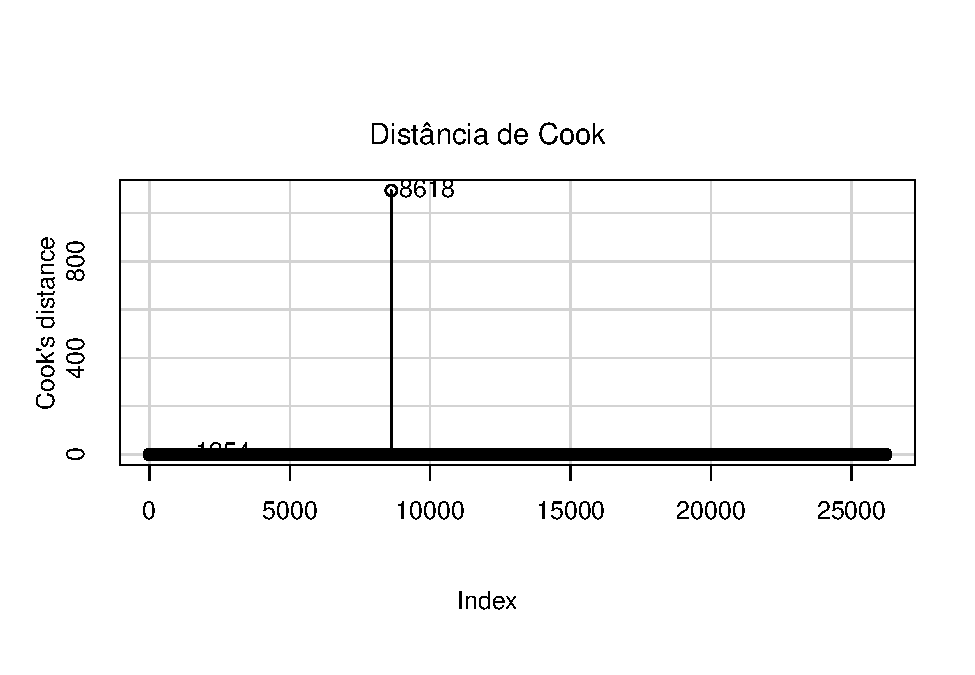
\includegraphics{Dados_Binários1_files/figure-latex/unnamed-chunk-17-1.pdf}

\textbf{5.4 Medidas de Influencia}

\begin{Shaded}
\begin{Highlighting}[]
\KeywordTok{influenceIndexPlot}\NormalTok{(ajuste4}\FloatTok{.1}\NormalTok{, }\DataTypeTok{vars=}\KeywordTok{c}\NormalTok{(}\StringTok{"Cook"}\NormalTok{), }\DataTypeTok{main=}\StringTok{"Distância de Cook"}\NormalTok{)}
\end{Highlighting}
\end{Shaded}

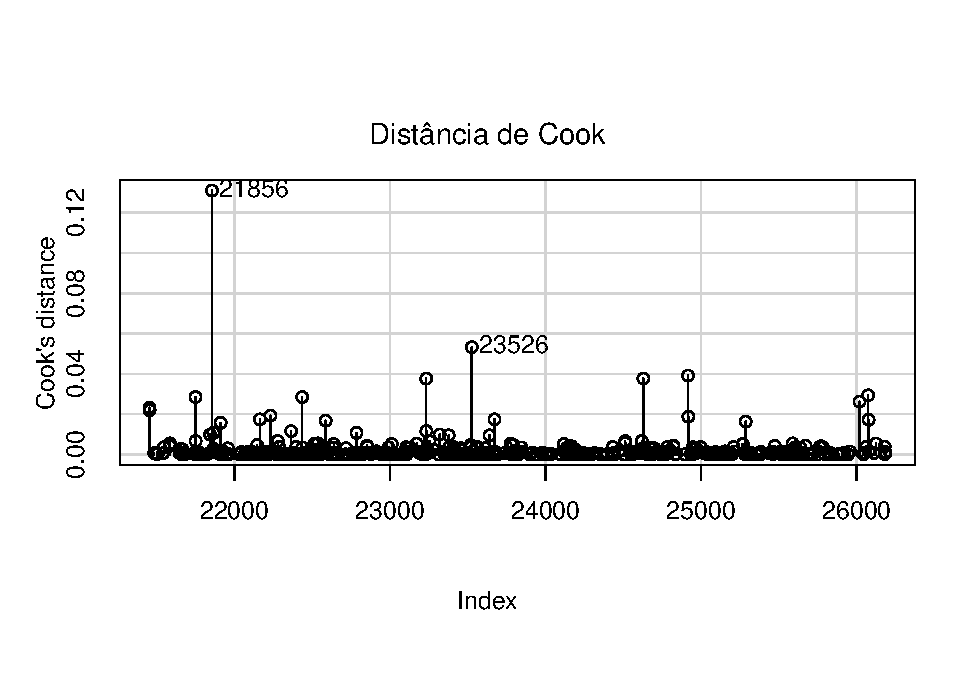
\includegraphics{Dados_Binários1_files/figure-latex/unnamed-chunk-18-1.pdf}

\begin{Shaded}
\begin{Highlighting}[]
\KeywordTok{influenceIndexPlot}\NormalTok{(ajuste4}\FloatTok{.1}\NormalTok{, }\DataTypeTok{vars=}\KeywordTok{c}\NormalTok{(}\StringTok{"Studentized"}\NormalTok{), }\DataTypeTok{main=}\StringTok{"Resíduos Padronizados"}\NormalTok{)}
\end{Highlighting}
\end{Shaded}

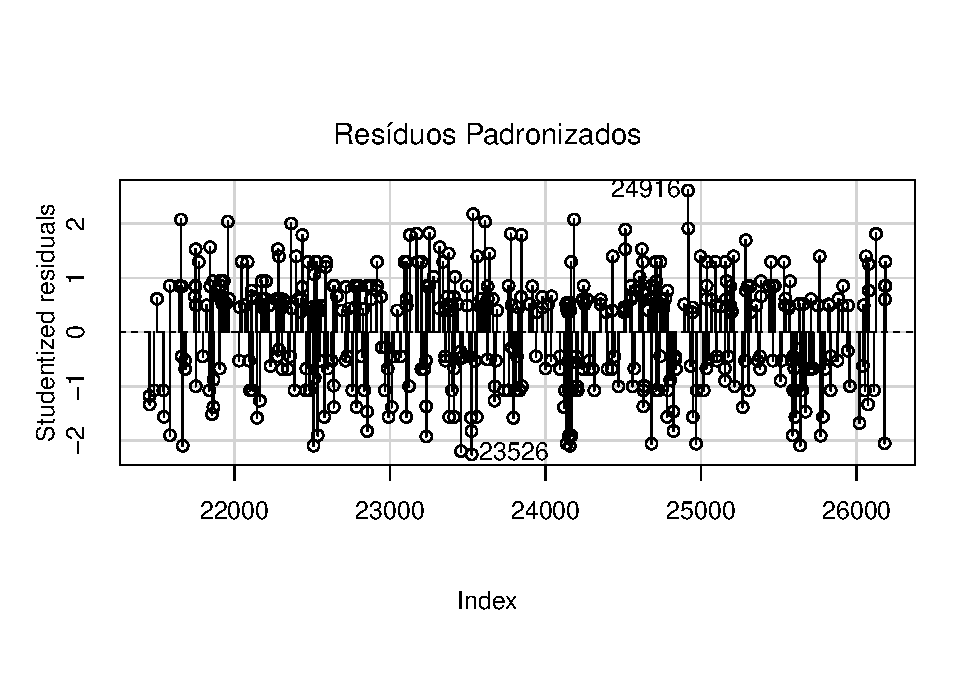
\includegraphics{Dados_Binários1_files/figure-latex/unnamed-chunk-19-1.pdf}

\textbf{5.5 Resíduos Quantílicos Aleatoriazados}

\textbf{5.7 Gráficos de Efeitos}

\begin{Shaded}
\begin{Highlighting}[]
\KeywordTok{plot}\NormalTok{(}\KeywordTok{allEffects}\NormalTok{(ajuste4}\FloatTok{.1}\NormalTok{), }\DataTypeTok{type =} \StringTok{'response'}\NormalTok{, }\DataTypeTok{main =} \StringTok{''}\NormalTok{)}
\end{Highlighting}
\end{Shaded}

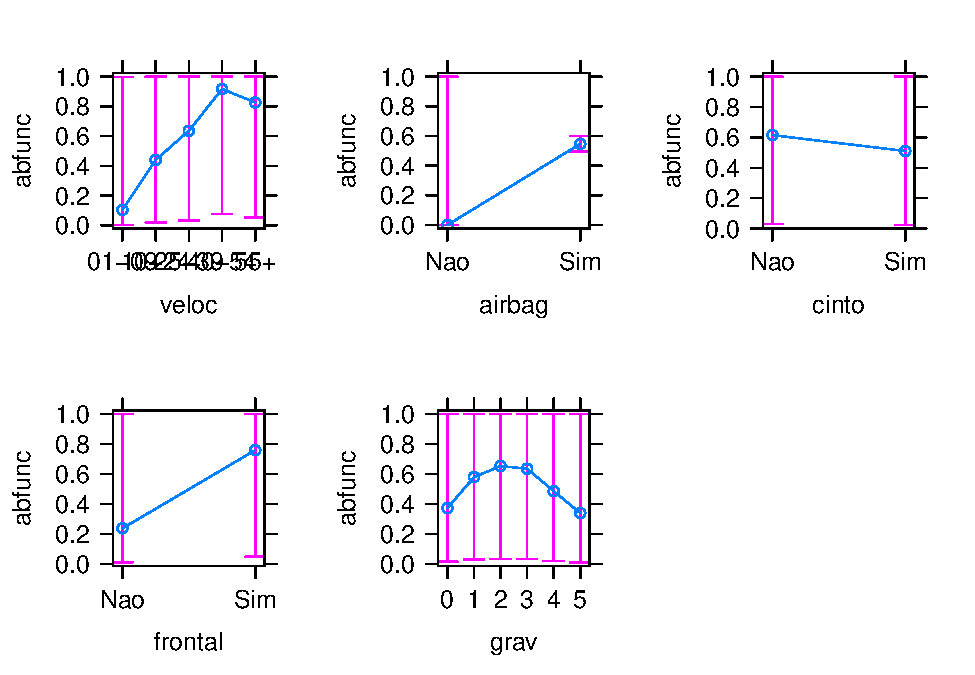
\includegraphics{Dados_Binários1_files/figure-latex/unnamed-chunk-20-1.pdf}

\section{6. PREDIÇÃO}\label{predicao}

\section{7. AVALIAÇÃO DO PODER PREDITIVO DO
MODELO}\label{avaliacao-do-poder-preditivo-do-modelo}

\textbf{7.1 Divisão da Base de dados}

\textbf{7.2 Ponto de Corte}

\textbf{7.3 Sensibilidade e Especificidade}

\textbf{7.4 Curva ROC}

\textbf{7.5 Outra Alternativa de validação}

\section{8. REFERÊNCIAS}\label{referencias}

\section{}\label{section}


\end{document}
